\chapter{Least Squares Problem: Multi-way Choice \normalfont{\emoji{motorway}}}

Nel capitolo precedente l'algoritmo richiedeva una ricorsione basata su scelte
binarie, in questo capitolo invece introdurremo un algoritmo che richiede ad
ogni step un numero di scelte polinomiali (\textit{multi-way choice}). Vedremo
come la programmazione dinamica si presta molto bene a risolvere questi
problemi.

\section{Linear Least Square}

\subsection{Il Problema}

La formulazione del problema è la seguente:

\paragraph*{} dato un insieme $P$ composto di $n$ punti sul piano denotati con\\
$(x_1, y_1), (x_2, y_2), \ldots, (x_n, y_n)$; e supponiamo che $x_1 < x_2 <
    \ldots < x_n$ (sono strettamente crescenti). Data una linea $L$ definita
dall'equazione $y = ax + b$, definiamo l'\textit{errore} di $L$ in funzione
di $P$ come la somma delle distanze al quadrato della linea rispetto ai
punti in $P$. Formalmente:
\[
    Error(L, P) = \sum_{i=1}^{n} (y_i - ax_i - b)^2
\]

\begin{figure}[H]
    \centering
    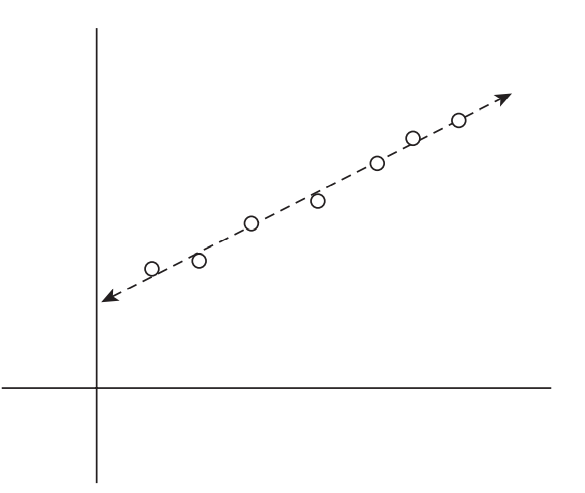
\includegraphics[width=6cm, keepaspectratio]{capitoli/imgs/linear_least.png}
    \caption{Esempio di una tipica istanza e soluzione del problema
        \textit{Linear Least}}
\end{figure}

\subsection{\goal}

È intuibile che il goal dell'algoritmo è quello di cercare la linea con errore
minimo, che può essere facilmente trovata utilizzando l'analisi matematica.
La linea di errore minimo è $y = ax + b$ dove:

\[
    a = \frac{n \sum_{i} x_i y_i - (\sum_{i} x_i) (\sum_{i} y_i)}{n \sum_{i} x_i^2 - (\sum_{i} x_i)^2} \ \ \  \ \ b = \frac{\sum_{i} y_i - a \sum_{i} x_i}{n}
\]

\section{Segmented Least Square}

Le formule appena citate sono utilizzabili solo se i punti di $P$ hanno un
andamento che è abbastanza lineare ma falliscono in altre circostanze.

\begin{figure}[H]
    \centering
    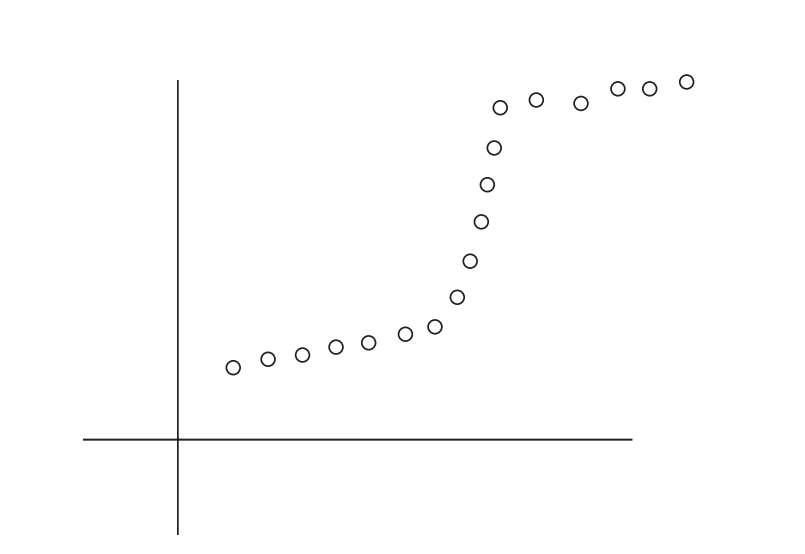
\includegraphics[width=8cm, keepaspectratio]{capitoli/imgs/segmente_linear_least.png}
    \caption{Esempio di funzione non risolvibile con Linear Least Square}
\end{figure}

Come è evidente (\textit{lapalissiano \normalfont{\emoji{gem}}}) dalla figura
non è possibile trovare una linea che approssimi in maniera soddisfacente i
punti, dunque per risolvere il problema possiamo pensare di rilassare la
condizione che sia solo una la linea. Questo però implica dover riformulare il
goal che altrimenti risulterebbe banale (si fanno $n$ linee che passano per ogni
punto).

\subsection{Costi}

La parte che computa gli errori ha costo in tempo $O(n^3)$ (si può portare a
$O(n^2)$).
La parte che trova il valore ottimo ha costo $O(n^2)$.\\

In spazio l'algoritmo ha costo $O(n^2)$ ma può essere ridotto a $O(n)$

\subsection{\goal}

Formalmente, il problema è espresso come segue:

\paragraph*{} come prima abbiamo un set di punti $P = \{(x_1, y_1), (x_2, y_2),
    \ldots, (x_n, y_n)\}$ strettamente crescenti. Denoteremo l'insieme dei punti
$(x_i, y_i)$ con $p_i$. Vogliamo partizionare $P$ in un qualche numero di
segmenti, ogni numero di segmenti è un sottoinsieme di $P$ che rappresenta un
\textit{set} contiguo delle coordinate $x$ con la forma $\{p_i, p_{i+1}, \ldots,
    p_{j-1}, p_j\}$ per degli indici $i \leq j$. Dopodiché, per ogni segmento $S$
calcoliamo la linea che minimizza l'errore rispetto ai punti in $S$ secondo
quanto espresso dalle formule enunciate prima.\\

Definiamo infine una penalità per una data partizione come la somma dei seguenti
termini:

\begin{itemize}
    \item Numero di segmenti in cui viene partizionato $P$ moltiplicato per un
          valore $C > 0$ (più è grande e più penalizza tante partizioni)
    \item Per ogni segmento l'errore della linea ottima attraverso quel
          segmento.
\end{itemize}


Il goal del Segmented Least Square Problem è quindi quello di trovare la
partizione di \textbf{penalità minima}.

\subsection{Funzionamento}

Per come è fatta la programmazione dinamica noi vogliamo suddividere il problema
in sotto-problemi e per farlo partiamo dall'osservazione che l'ultimo punto
appartiene ad una partizione ottima che parte da un valore $p_i$ fino a $p_n$ e
che possiamo togliere questi punti dal totale per ottenete un sotto-problema più
piccolo. Supponiamo che la soluzione ottima sia denotata da \verb|OPT(j)|, per i
punti che vanno da $p_1$ a $p_j$, allora avremo che la soluzione ottima al
problema dato l'ultimo segmento che va da $p_i$ a $p_n$, sarà dalla seguente
formula:

\[
    OPT(n) = e_{i,n} + C + OPT(i - 1)
\]

Questa formula è data dalla soluzione ottima dell'ultima partizione ($e_{i,n} + C$)
a cui viene aggiunta la soluzione ottima di tutte le partizioni precedenti
($OPT(i -1)$). Per i sotto-problemi possiamo scrivere la soluzione al problema
in forma ricorsiva utilizzando la formula appena espressa che prenderà la forma:

\[
    OPT(j) = \min_{1 \leq i \leq j}(e_{i,j} + C + OPT(i - 1))
\]

Possiamo ora dare una versione di questo algoritmo in pseudocodice:

\begin{lstlisting}[language=Javascript]
    function Segmented-Least-Squares(n) {
        M[0 ... n]
        M[0] = 0

        // compute the errors
        for (j in 1 ... n) {
            for (i in 1 ... j) {
                compute eij for the segment pi, ..., pj
            }
        }

        // find optimal value
        for (j in 1 ... n) {
            M[j] = min_i(eij + C + M[i - 1]) // OPT(J)
        }

        return M[n]
    }
\end{lstlisting}

Dopo aver trovato la soluzione ottima, possiamo sfruttare la memoization per
ricavarci i segmenti in tempi brevi.

\begin{lstlisting}[language=Javascript]
    function Find-Segments(j) {
        if (j == 0) print('')

        else {
            Find an i that minimizes ei,j + C + M[i − 1]
            Output the segment {pi,..., pj} and the result of Find-Segments(i − 1)
        }
    }
\end{lstlisting}

L'algoritmo ha costo $O(n^3)$ in tempo e $O(n^2)$ in spazio.
Questo tempo può essere ridotto applicando la memoization alle formule per il calcolo
dell'errore viste in precedenza portandolo a $O(n^2)$ per il tempo e $O(n)$ per lo spazio.